% !TEX TS-program = xelatex
%
\documentclass[ngerman]{scrartcl}

\usepackage[ngerman]{babel}
\usepackage{amsmath}
\usepackage{enumitem}

\usepackage{siunitx}
\sisetup{per-mode = symbol, binary-units = true}
\DeclareSIUnit\mbyte{Byte}

\usepackage{graphicx}

\begin{document}

\section*{1}
	\begin{enumerate}[label=\alph*)]
    \item
    Abbildung mit eingefügten Werten:

    \begin{figure}[ht]
      \centering
      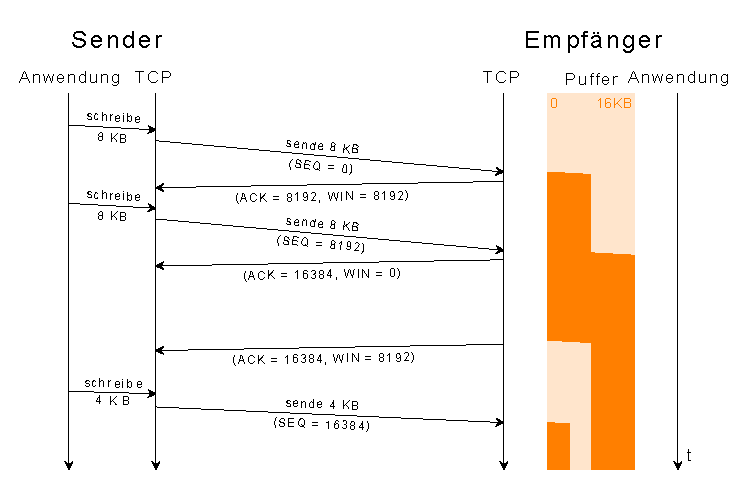
\includegraphics{uebung6-1a.pdf}
    \end{figure}

    \item
    Der Puffer des Empfängers ist \SI{16}{\kilo\byte} groß.

    \item
    Die vom Sender übertragene Datenmenge ist \SI{20}{\kilo\byte} groß.

    \item
    Der Sender könnte dann zuerst \SI{16}{\kilo\byte} übertragen, und danach sofort die restlichen \SI{4}{\kilo\byte}.

    \newpage

    \item
    Annahmen:
      \begin{itemize}
        \item
        \item
        \item
      \end{itemize}

    \begin{figure}[ht]
      \centering
      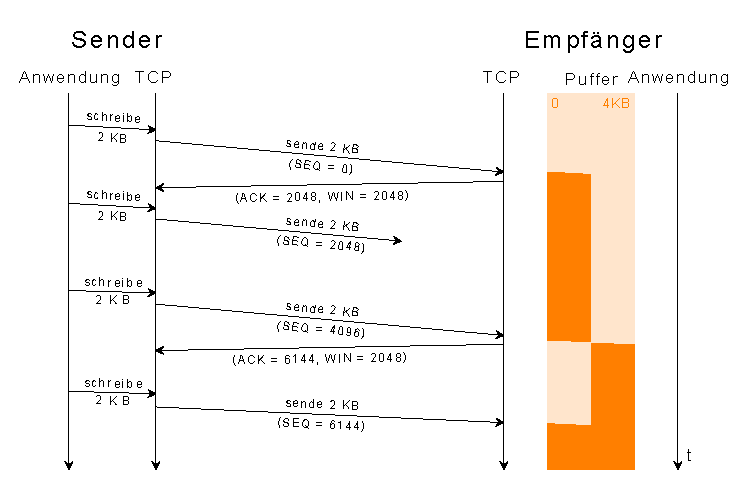
\includegraphics{uebung6-1e.pdf}
    \end{figure}
  \end{enumerate}
\end{document}
